\chapter{Evaluierung und Weiterentwicklung} \label{sec:evaluierung}

Folgendes Kapitel beinhaltet eine Evaluierung der verwendeten Methoden, Probleme und mögliche Optimierungsansätze in Bezug zur Objekterkennung. Verbesserungen der Handhabung sind in der Arbeit von Steinbeck aufgeführt \cite[Abschnitt~5]{steinbeck_entwicklung_2022}.

\section{Auswertung und Optimierung}

Die Verwendung von \textit{\ac{DL}} mit dem \textit{YOLOv3 Tiny}-Algorithmus ist aufgrund der für ein \textit{\ac{CNN}} sehr schnellen Klassifizierung und Positionserkennung auch mit schwacher Hardware und der ausreichenden Genauigkeit gut für die Anwendung geeignet. Auch die sehr geringe Fehlerrate trotz des kleinen Datensatzes zum Einlernen mit \textit{Darknet} spricht für \textit{\ac{DL}} und gegen die mit höherem Aufwand verbundenen Verwendung traditioneller \textit{\ac{CV}}. \textit{YOLO} kann außerdem mit dem Paket \textit{darknet\_ros}, für das schon Versionen für die Verwendung von \ac{ROS}-II verfügbar sind, gut in \ac{ROS} integriert werden. Aufgrund dieser Verfügbarkeit und der aktiven Entwicklung ist eine zukünftige Weiterentwicklung des \textit{rv6l\_3d}-Pakets gut umsetzbar. Wegen der Verfügbarkeit von \textit{Packages} wie \textit{darknet\_ros\_3d} ist die Verwendung der \ac{ROS}-Version \textit{Noetic} aktuell für die Anwendung geeignet. Mit der Nutzung der Intel RealSense als Alternative zur Microsoft Kinect kann aufgrund der Möglichkeit einer Befestigung am Endeffektor bei guter Ausrichtung dieser eine hohe Genauigkeit durch Ausgleichen der Positionsabweichung des verwendeten Roboters erzielt werden. Die Objekte können wegen der guten Kalibrierung ab Werk und des integrierten Infrarotprojektors sehr genau lokalisiert werden. Auch die Treiberunterstützung bietet mit Bereitstellung der Daten in \textit{OpenNI} kompatiblem Format Vorteile gegenüber anderen 3D-Kamerasystemen. Durch die zweistufige Mittelpunkterkennung kann der Zielpunkt sehr genau angefahren werden. Die Abweichung in $z$-Richtung ist hier minimal. Wegen Toleranzen bei der Befestigung der Kamera am Endeffektor können beispielsweise aufgrund einer Neigung Abweichungen in der $x$-$y$-Ebene entstehen. In den durchgeführten Tests waren diese allerdings gering und führten somit nicht zu Problemen. Die Kommunikation zwischen allen verwendeten \textit{Packages} funktioniert auch bei Nutzung verschiedener Programmiersprachen problemlos.

Auch wenn die Erkennungsrate durch den \textit{\ac{YOLO}}-Algorithmus bei den verwendeten Objekten sehr hoch ist, können vor allem bei ähnlichen Teilen Fehler bei der Klassifizierung auftreten. Mit der Verwendung eines größeren Datensatzes, einer Erhöhung von Auflösung oder Iterationen, oder Optimierungen des bestehenden Datensatzes kann die Erkennungsrate und Positionsgenauigkeit gesteigert werden. Die um $90$° gegenüber dem Endeffektor rotierte Montage ist aufgrund der Nähe zu einer Singularität des RV6L durch einen gestreckten Arm, bei dem die Achsen $4$ und $6$ deckungsgleich sind, in der maximalen Höhe limitiert. Eine Montage mit Blickrichtung parallel zum Kontaktpunkt des verwendeten Endeffektors würde diese Problematik lösen, jedoch den für die Kamera erreichbaren Bereich in $x$-Richtung des Basiskoordinatensystems verkleinern. Zur Optimierung der Genauigkeit in der $x$-$y$-Ebene kann eine Hand-Auge-Kalibrierung durchgeführt werden. Die Genauigkeit in $z$-Richtung wird auch hier nur wenig durch den Kamerawinkel beeinflusst.

\section{Ansätze zur Weiterentwicklung des rv6l\_3d-Pakets}

Während die Grundfunktionalität zur Objekterkennung und Positionserkennung gegeben ist, ist eine Weiterentwicklung des \textit{rv6l\_3d} Pakets notwendig. Aktuell funktioniert die Schnittstelle zwischen den Objekterkennungs- und Handhabungspaketen nur teilweise, da der \textit{Bounding Box Subscriber} \seeAtt{sec:handhabung} trotz Erkennung aller Bauteile nur die Position des zuletzt erkannten Blocks an das Programm zur Handhabung weitergibt. Somit wird eine Logik zur gleichzeitigen Weitergabe aller ungefähren Positionen der ersten Scanposition benötigt. Außerdem ist für die zweite Position eine Logik notwendig, die bei mehreren Teilen im Erkennungsbereich das mittlere Objekt identifiziert und nur dessen Position an den \textit{Subscriber} weitergibt. Somit ist die Erkennung und Aufnahme des korrekten Objekts gewährleistet. 
Zur Optimierung des Systems können außerdem folgende Ansätze genutzt werden: Aktuell ist der Erkennungsbereich durch den maximalen Aufnahmebereich des Kamerasystems limitiert, da der erste Scanvorgang des kompletten Bereichs nur mit fester Kameraposition durchgeführt wird. Dieses Problem kann durch die Implementierung einer Bewegung parallel zur $x$-$y$-Ebene des Basiskoordinatensystems während des Scans und anschließender Umrechnung der Objektpositionen in vom Handhabungsprogramm nutzbare Werte gelöst werden, wobei jedoch die durch die Perspektive abweichende Mittelpunktposition der Objekte beachtet werden muss. Auch eine Erkennung aus unterschiedlichen Kameraorientierungen oder ein von der Objektgröße abhängiger Abstand zwischen Kamera und Bauteil ist denkbar. Bei entsprechender Leistung des zur Bilderkennung verwendeten Computers ist ein Anfahren des Objekts mit Abgleich zwischen Kamera- und Objektmittelpunkt in Echtzeit zur Steigerung der Genauigkeit in $x$-$y$-Ebene möglich. Auch wenn der Mittelpunkt bei den verwendeten Objekten eine sinnvolle Greifposition darstellt, ist dieser nicht in allen Anwendungsfällen optimal. Eine Alternative ist etwa die Erkennung des höchsten Punktes eines Objekts oder einer geraden Fläche. Zur Verringerung der Fehleranfälligkeit kann zudem die Ablagehöhe für das Bauteil in der Zielposition gemessen werden, um Kollisionen mit Objekten im Ablagebereich zu vermeiden. Ein weiterer wichtiger Aspekt ist die Implementierung von Funktionen zur Ausnahmebehandlung. Wird beispielsweise ein Block nicht erkannt, kommt es beim Bewegungsprogramm in der aktuellen Form zu einem Fehler. Ein möglicher Lösungsansatz ist hier die Nutzung der 3D-\textit{Point Cloud}, um durch Erhöhungen im Bauraum Objekte zu erkennen und einen erneuten Scanvorgang zu starten. Auch die Erkennung von mehr Teilen, als im Bauplan genutzt werden, kann zu unvorhersehbaren Ereignissen beim Ausführen des Paktes führen.

Ein Nachteil des \textit{\ac{YOLO}}-Algorithmus ist die fehlende Unterstützung für \textit{\ac{OBBs}}. Stattdessen werden \textit{\ac{HBBs}} verwendet, die immer aus horizontalen und vertikalen Kanten ohne eine Möglichkeit zur Orientierungserkennung bestehen. Somit muss für eine Erkennung der Bauteilorientierung ein anderer Algorithmus genutzt werden. Dazu kann beispielsweise der Ansatz von Yin et al. zur Kalkulation von \textit{\ac{OBBs}} basierend auf \textit{\ac{YOLO}} genutzt werden \seeFig{fig:yolo_hbb_obb} \cite{yin_fast_2018}.

\begin{figure}[ht]
    \centering
    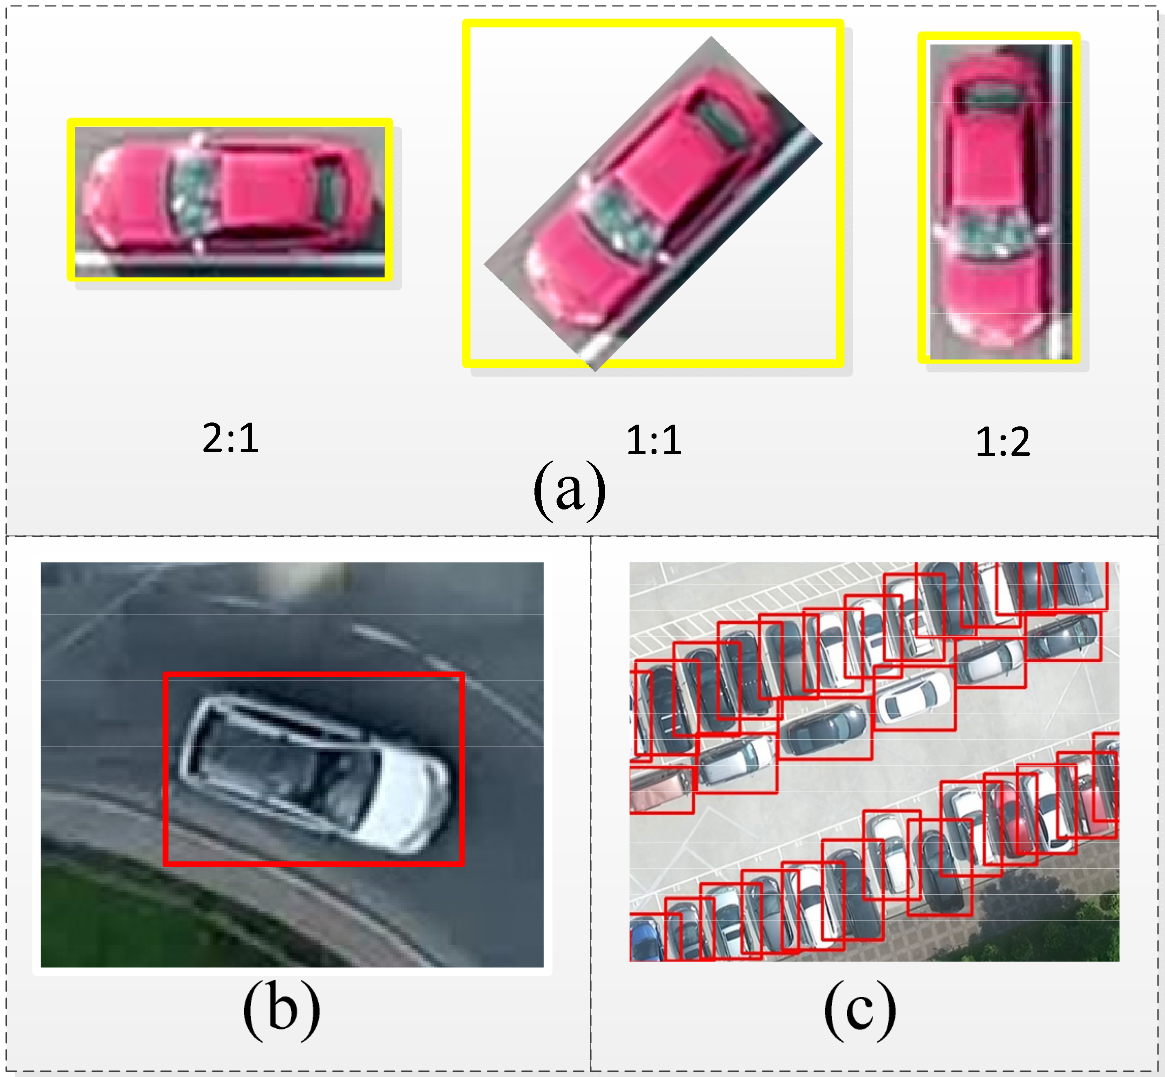
\includegraphics[height=6.29cm]{Bilder/yolo_hbb.png}
    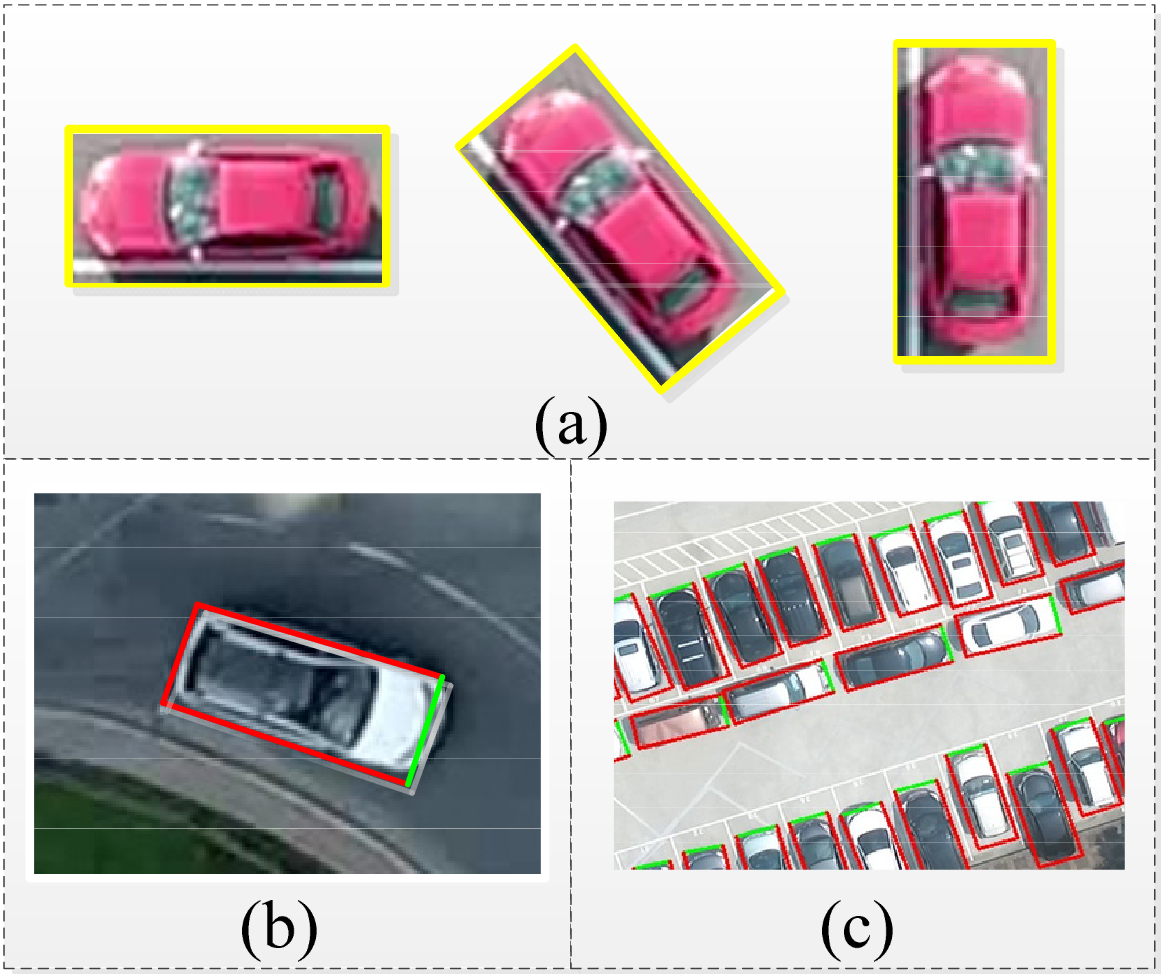
\includegraphics[height=6.29cm]{Bilder/yolo_obb.png}
    \caption{Vergleich zwischen HBBs (links) und OBBs (rechts) \cite{yin_fast_2018}}
    \label{fig:yolo_hbb_obb}
\end{figure}

Eine Implementierung von \textit{YOLOv5} mit \textit{\ac{OBBs}}, die ein Paket für die Nutzung mit \ac{ROS} beinhaltet, wurde im Dezember 2021 unter dem Namen "RoSA: Cube Detector" veröffentlicht \cite{hempel_rosa_2021}.

Eine weitere Optimierung besteht in der Kollisionsvermeidung mit erkannten Objekten. Der genutzte Bahnplanungsalgorithmus umfährt bekannte Objekte im Bauraum. Jedoch werden die erkannten Bauteile diesem nicht zur Verfügung gestellt. Die Bereitstellung der Kollisionsobjekte kann entweder über Einfügen der bekannten Objekte an den durch die Objekterkennung ermittelten Mittelpunktpositionen in die Simulation oder der Nutzung der von der Kamera generierten \textit{Point Cloud} umgesetzt werden.